\documentclass[a4paper]{article}
\usepackage{geometry}
\usepackage{multicol}
\usepackage{setspace}
\usepackage{listings}
\usepackage{graphicx}
\usepackage{algorithm}
\usepackage{algpseudocode}
\usepackage{amsmath}
\usepackage{amssymb}
\usepackage{multicol}
\usepackage{float}
\DeclareGraphicsExtensions{.eps,.ps,.jpg,.bmp}
\usepackage{xcolor}
%\setlength{\parskip}{0.5\baselineskip}
\geometry{left=3.0cm,right=2.0cm,top=1.5cm,bottom=2.0cm} 
\title{\textbf{Algorithmn HW6}}
\author{5140379032 JIN YI FAN}
\date{}
\begin{document}
\maketitle
\begin{spacing}{1.3}
%\begin{multicols}{2}
\section*{Problem 9.16}
\begin{figure}[H]
    \centering
    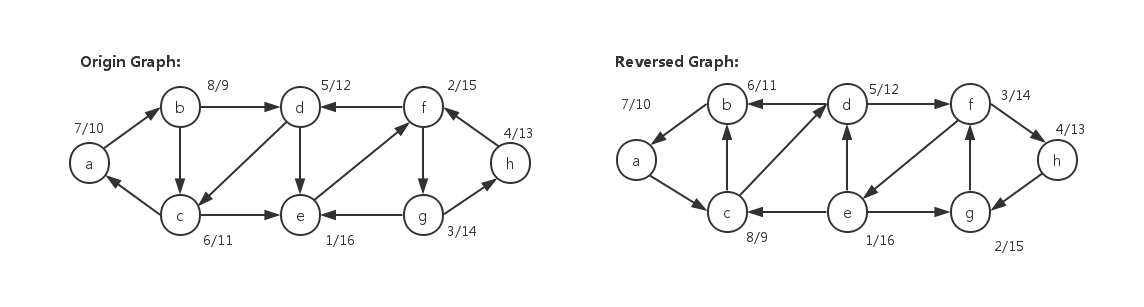
\includegraphics[width=15cm]{graph.png}
\end{figure}
Firstly, apply DFS and update the $post$ value;
\\Secondly, reverse graph $G$ to $G^T$;
\\Thirdly, apply DFS to $G^T$ starting at vertex with maximum $post$ value, $e$ this time;
\\A single DFS of this $G^T$ can approach all the vertexes, so the whole graph $G$ is strongly connected.
\section*{Problem 9.32}
\begin{algorithmic}[1]
\Require a given graph $G=(V,E)$
\Ensure whether it is a bipartite graph
\Function{dfs}{v}
\State mark $v$ visited
\State $v.mark\gets (color\gets !color)$\Comment{mark neighbour vertexes with different colors}
\For{each edge $(v,w)\in E$}
\If{$w$ is marked unvisited} 
\State \Call{dfs}{w}
\State \textbf{return} $True$
\Else \State \textbf{return} ($w.mark==v.mark?$) $False$ : $True$
\EndIf
\EndFor
\EndFunction
\State $color\gets 1$\Comment{main function}
\State mark each vertex $v\in V$ unvisited
\For{each vertex $v\in V$ marked unvisited}\Comment{start dfs}    
\If{\Call{dfs}{v}==$False$}
\State \textbf{return} $False$
\EndIf
\EndFor
\State \textbf{return} $True$
\end{algorithmic}
This is an $O(V+E)$ algorithm

\section*{Reverse graph}
\begin{algorithmic}[1]
\Require a directed graph $G=(V,E)$
\Ensure the reversed graph $G^T=(V,E^R)$
\For{each edge $(v,u)\in E$}
\State append $(u,v)$ to $E^R$
\EndFor
\State replace $E$ with $E^R$
\end{algorithmic}

\section*{Find a cycle}
\begin{algorithmic}[1]
\Require an undirected graph $G=(V,E)$, $e=(u,v)\in E$
\Ensure whether $G$ has a cycle containing $e$
\State delete $e$ from $E$
\State apply \Call{DFS}{} to $G$ with $pre/post$ signature
\If{$v.pre>u.post$ or $u.pre>v.post$} \Comment{exist such cycle iff $u$ and $v$ are still in same component}
\State \textbf{return} $False$\Comment{which means there shouldn't have any cross edge between them}
\Else
\State \textbf{return} $True$
\EndIf
\end{algorithmic}

\section*{Hamiltonian path in a DAG}
\begin{algorithmic}[1]
\Require a DAG $G=(V,E)$
\Ensure whether it has a Hamiltonian path
\State $topo[]\gets$ the topological sorted vertex sequence of $G$
\For{$i\gets 1$ to $topo.size$}\Comment{whether every consecutive pairs are connected}
\State find the edge between $topo[i-1]$ and $topo[i]$ in $E$
\If{cannot found} \Comment{once unconnected, there won't exist}
\State \textbf{return} $"can\ not\ find"$
\EndIf
\EndFor
\State \textbf{return} $topo$ \Comment{the topological sort sequence is actually the Hamiltonian Path}
\end{algorithmic}
%\end{multicols}
\end{spacing}
\end{document}

